\documentclass[11pt]{article}

\usepackage{amsmath}
\usepackage{amssymb}
\usepackage{color}
\usepackage{graphicx}
\usepackage{listings}
\usepackage{xcolor}
\usepackage{cancel}

\definecolor{codegreen}{rgb}{0,0.6,0}
\definecolor{codegray}{rgb}{0.5,0.5,0.5}
\definecolor{codepurple}{rgb}{0.58,0,0.82}
\definecolor{backcolour}{rgb}{0.95,0.95,0.92}

\lstdefinestyle{mystyle}
{
    backgroundcolor=\color{backcolour},   
    commentstyle=\color{codegreen},
    keywordstyle=\color{magenta},
    numberstyle=\tiny\color{codegray},
    stringstyle=\color{codepurple},
    basicstyle=\ttfamily\footnotesize,
    breakatwhitespace=false,         
    breaklines=true,                 
    captionpos=b,                    
    keepspaces=true,                 
    numbers=left,                    
    numbersep=5pt,                  
    showspaces=false,                
    showstringspaces=false,
    showtabs=false,                  
    tabsize=2
}

\lstset{style=mystyle}

\textwidth=6.5in
\textheight=9in
\topmargin=-0.8in
\headheight=15.75pt
\headsep=.35in
\oddsidemargin=0.0in
\evensidemargin=0.0in

\newcommand{\bu}{{\bf u}}
\newcommand{\bv}{{\bf v}}
\newcommand{\bw}{{\bf w}}
\newcommand{\dx}{{\Delta x}}
\newcommand{\dt}{{\Delta t}}
\newcommand{\bra}[1]{\left(#1\right)}

\begin{document}
\begin{flushright}
\small{MATH-6840\\
Vignesh Ramakrishnan\\
{\bf Due: Monday April 18, 2022}}
\end{flushright}

\begin{center}
\large{Problem Set 9}\\
\end{center}

\begin{enumerate}
  %%%%%
  %%%%%
  %%%%%
  %%%%%
  %%%%%
  \item {\color{red}(20 pts.) Consider the linear hyperbolic system}
    \[
      \bu_t+A\bu_x=0
    \]
  
    {\color{red}where $A$ is a constant coefficient matrix. Now introduce the upwind method}
    \[
      \bv_j^{n+1}=\bv_j^n-A_{+}\frac{\dt}{\dx}\left(\bv_j^n-\bv_{j-1}^n\right)-A_{-}\frac{\dt}{\dx}\left(\bv_{j+1}^n-\bv_{j}^n\right)
    \]
    {\color{red}where $A_{\pm}$ are the matrices constructed using the positive/negative eigenvalues and $A=A_{+}+A_{-}$ as discussed in class. For each $A$ given below do the following}
    \begin{enumerate}
    %%%
    %%%
    %%%
      \item {\color{blue}Find the matrices $A_{+}$ and $A_{-}$ in the upwind method above.} \\
      \[
        A=
        \begin{bmatrix}
          3 & 1 \\
          1 & 3
        \end{bmatrix}
        \qquad \qquad
        A=
        \begin{bmatrix}
        2 & 3 & -3\\
        1 & 2 & -1\\
        1 & 3 & -2
        \end{bmatrix}
      \]      
      \begin{align*}
          Av &= \ \lambda v \\
          (A-\lambda I)v &= \ 0
      \end{align*}
      \begin{align*}
          \begin{bmatrix}
          3-\lambda & 1 \\
          1 & 3-\lambda
          \end{bmatrix}v =& 0 & 
          \begin{bmatrix}
          2-\lambda & 3 & -3 \\
          1 & 2-\lambda & -1 \\
          1 & 3 & -2-\lambda
          \end{bmatrix}v =& 0 \\
      \end{align*}
      The characteristic equations are
      \begin{align*}
          (\lambda-3)^2 -1 =& \ 0 & -(\lambda-2)\bra{\lambda^2-1}+3(\lambda+1)-3\bra{\lambda+1}=& \ 0 \\
          \lambda =& \  2,4 & \lambda =& \ 2,1,-1 
      \end{align*}
      Using these $\lambda$'s we can find out the eigen-vectors as follows,
      \begin{align*}
          (\lambda=2), \ 
          \begin{bmatrix}
          1 & 1 \\
          1 & 1
          \end{bmatrix}v =& \ 0 &
          (\lambda=4), \ 
          \begin{bmatrix}
          -1 & 1 \\
          1 & -1
          \end{bmatrix}v =& 0 
      \end{align*}
      Therefore, $R = 
      \begin{bmatrix}
      1 & 1 \\
      -1 & 1
      \end{bmatrix}$ which contains the eigen-vectors as its column entries.\\
      Similar procedure is followed for the second case and $R = 
      \begin{bmatrix}
      -1 & 0 & 1 \\
      -1 & 1 & 0 \\
      -1 & 1 & 1
      \end{bmatrix}$. \\
      Now, the eigenvalue decomposition of square matrix $A = R\Lambda R^{-1}$, where, $\Lambda$ is a diagonal matrix containing the eigen-values.\\
      \begin{align*}
        \Lambda =& \
          \begin{bmatrix}
          2 & 0 \\
          0 & 4 
          \end{bmatrix} & 
        \Lambda =& \ 
        \begin{bmatrix}
        2 & 0 & 0\\
        0 & 1 & 0\\
        0 & 0 & -1
        \end{bmatrix}
      \end{align*}
      This can be split up and written as $\Lambda^{+}$ and $\Lambda^{-}$ such that $\Lambda = \Lambda^+ + \Lambda^-$.
      \begin{align*}
          \Lambda^{+} =& \ 
          \begin{bmatrix}
          2 & 0 \\
          0 & 4
          \end{bmatrix} & 
          \Lambda^{+} =& \
          \begin{bmatrix}
          2 & 0 & 0 \\
          0 & 1 & 0 \\
          0 & 0 & 0 
          \end{bmatrix} \\
          \Lambda^{-} =& \ 
          \begin{bmatrix}
          0 & 0 \\
          0 & 0
          \end{bmatrix} & 
          \Lambda^{-} =& \ 
          \begin{bmatrix}
          0 & 0 & 0 \\
          0 & 0 & 0 \\
          0 & 0 & -1
          \end{bmatrix}
      \end{align*}
      Therefore, 
      \begin{align*}
          A =& \ R\Lambda R^{-1} \\
          A =& \ R\bra{\Lambda^+ + \Lambda^-}R^{-1} \\
          A =& \ R\Lambda^{+}R^{-1} + R\Lambda^{-}R^{-1} \\
          A =& \ A^{+} + A^{-}
      \end{align*}
      \begin{align*}
          A^{+} =& \ 
          \begin{bmatrix}
          3 & 1 \\
          1 & 3
          \end{bmatrix} & 
          A^{+} =& \ 
          \begin{bmatrix}
          2 & 2 & -2 \\
          1 & 2 & -1 \\
          1 & 2 & -1
          \end{bmatrix} \\
          A^{-} =& \ 
          \begin{bmatrix}
          0 & 0 \\
          0 & 0 \\
          \end{bmatrix} & 
          A^{-} =& \ 
          \begin{bmatrix}
          0 & 1 & -1 \\
          0 & 0 & 0 \\
          0 & 1 & -1
          \end{bmatrix}
      \end{align*}
    %%%
    %%%
    %%%
    \item {\color{blue}If the PDE is defined for $x\in(-1,1)$ how many boundary conditions are needed at $x=-1$, and how many at $x=1$?} \\
    For the first case, we need two boundary conditions at $x=-1$ since both the eigenvalues are positive, which means the waves propagate from the left to right. No boundary condition is needed at $x=1$. \\
    For the second case, we need two boundary conditions at $x=-1$ and one at $x=1$, since we have 2 positive eigenvalues and one negative eigenvalue.
    %%%
    %%%
    %%%
    \item {\color{blue}Given BCs of the type just derived, determine an exact solution for the second of the two problems. Note that you may find it convenient to use either homogeneous or non-homogeneous BCs, it is your choice.}\\
    \begin{align*}
        \bu_t + A\bu_x =& \ \bf{0} \\
        R^{-1}\bu_t + R^{-1}R\Lambda R^{-1}\bu_x =& \ \bf{0} 
    \end{align*}
    Let $R^{-1}\bu = \bw$, then
    \begin{align*}
        \bw_t + \Lambda \bw_x =& \ \bf{0} \\
    \end{align*}
    These are three linear advection problems of the form 
    \begin{align*}
        w_t + cw_x =& \ 0
    \end{align*}
    $w = e^{-a\bra{x-ct+b}^2}$ is an exact solution to the PDE described above. 
    \begin{align*}
        w_t =& \ 2ac\bra{x-ct+b}e^{-a\bra{x-ct+b}^2} \\
        w_x =& \ -2a\bra{x-ct+b}e^{-a\bra{x-ct+b}^2}
    \end{align*}
    Hence,
    \begin{align*}
        w_t + cw_x =& \ 0
    \end{align*}
    Hence, the chosen exact solutions are
    \begin{align*}
        \bw =& \ 
        \begin{bmatrix}
        e^{-10\bra{x-\lambda_1t+0.1}^2} \\
        e^{-10\bra{x-\lambda_2t}^2} \\
        e^{-10\bra{x-\lambda_3t-0.1}^2}
        \end{bmatrix}
    \end{align*}
    where, $\lambda_1, \lambda_2$ and $\lambda_3$ are the eigenvalues of the matrix $A$. Two Dirchlet Boundary conditions at $x=-1$ for $\bw[0]$ and $\bw[1]$ are set up and one Dirchlet Boundary condition at $x=1$ for $\bw[2]$.
    %%%
    %%%
    %%%
    \item {\color{blue}Implement the upwind method with BCs. Use your exact solution from (c) to verify first-order convergence.}\\
    The domain is discretized with 2 ghost points on either ends of the domain. $\dx = 2/N$ and $x_j = -1+j\dx$ where $j=0,1,2,\ldots \ldots N$. \\
    The first order scheme is modified a little bit and written as, 
    \begin{align*}
        \bv_j^{n+1} = \bv_j^n - \Lambda^{+}\frac{\dt}{\dx}\bra{\bv_j^n - \bv_{j-1}^n} - \Lambda^{-}\frac{\dt}{\dx}\bra{\bv_{j+1}^n-\bv^n_j}   
    \end{align*}
    The Boundary conditions are written as,
    \begin{align*}
        \bv^n_{-1} =& \ 2\bf{\alpha}_1(t^n,-1) - \bv^n_{1} \\
        \bv^n_{N+1} =& \ 2\bf{\alpha}_2(t^n,1) - \bv^n_{N-1}
    \end{align*}
    Here, ${\bf \alpha}_1(t)$ is the vector of Left Boundary conditions and ${\bf \alpha}_2(t)$ is the vector of Right Boundary conditions. Then $\bu$ is recovered as $R\bw$. The error convergence plot is shown in Fig~\ref{fig:Q1_ErrPlot}.
    \begin{figure}[htp]
        \centering
        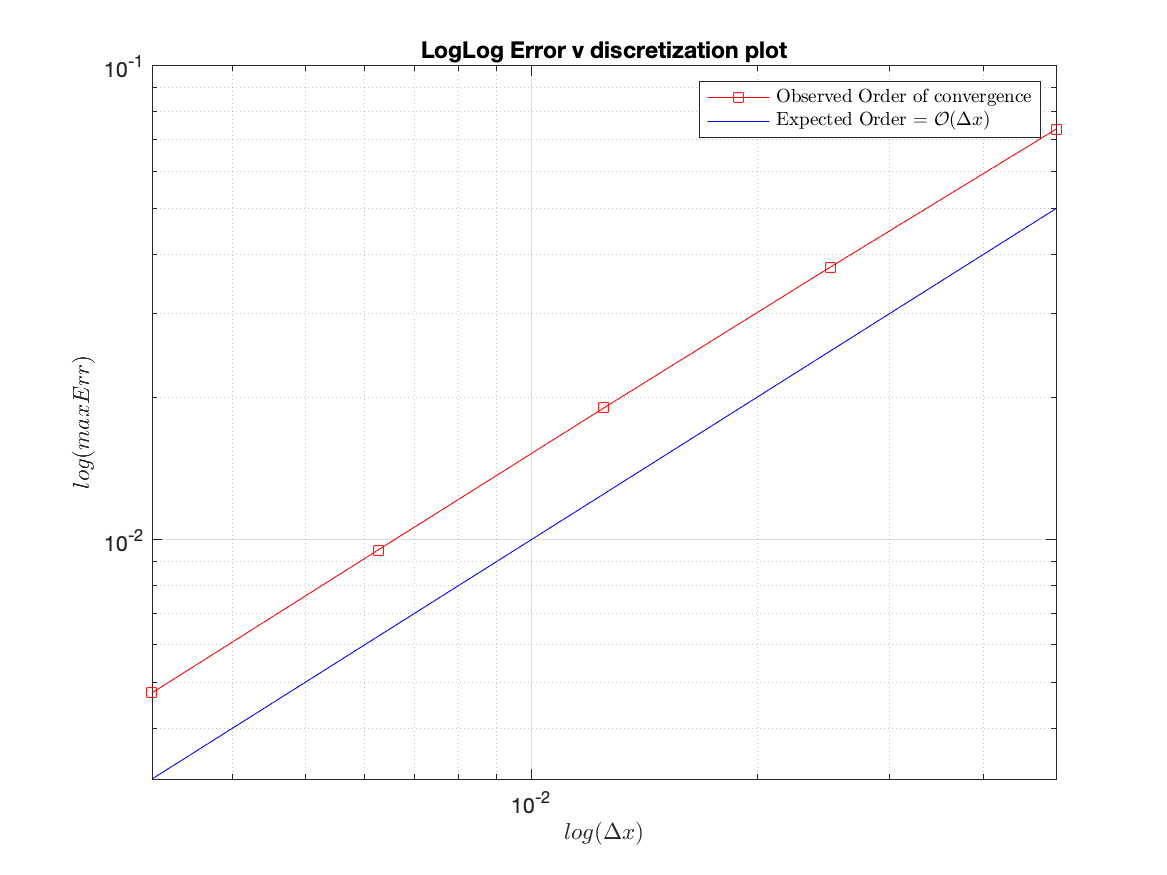
\includegraphics[width=4in]{Q1_ErrPlot.png}
        \caption{1st order convergence for Upwind-scheme}
        \label{fig:Q1_ErrPlot}
    \end{figure}
    %%%
    %%%
    %%%
    \item {\color{blue}(extra credit) Using a method-of-lines approach and RK-4, implement the standard centered second-order discretization for the original linear hyperbolic system. Use your exact solution from (c) to verify second-order convergence.} \\
    The second order scheme is written as, 
    \begin{align*}
        \frac{d\bv}{dt} =& \ -\Lambda^{+}\frac{\bv_{j+1}-\bv_{j-1}}{2\dx}-\Lambda^{-}\frac{\bv_{j+1}-\bv_{j-1}}{2\dx}
    \end{align*}
    The time integration scheme for this set of ODEs is RK-4 and it is formulated as follows, 
    \begin{align*}
        \bf{k}^1 =& \ -\Lambda^{+}\frac{\bv_{j+1}^n-\bv_{j-1}^n}{2\dx}-\Lambda^{-}\frac{\bv_{j+1}^n-\bv_{j-1}^n}{2\dx} \\
        \bf{k}^2 =& \ -\Lambda^{+}\frac{\bra{\bv_{j+1}^n+\frac{\dt}{2}\bf{k}^1_{j+1}}-\bra{\bv_{j-1}^n+\frac{\dt}{2}\bf{k}^1_{j-1}}}{2\dx}-\Lambda^{-}\frac{\bra{\bv_{j+1}^n+\frac{\dt}{2}\bf{k}^1_{j+1}}-\bra{\bv_{j-1}^n+\frac{\dt}{2}\bf{k}^1_{j-1}}}{2\dx} \\ 
        \bf{k}^3 =& \ -\Lambda^{+}\frac{\bra{\bv_{j+1}^n+\frac{\dt}{2}\bf{k}^2_{j+1}}-\bra{\bv_{j-1}^n+\frac{\dt}{2}\bf{k}^2_{j-1}}}{2\dx}-\Lambda^{-}\frac{\bra{\bv_{j+1}^n+\frac{\dt}{2}\bf{k}^2_{j+1}}-\bra{\bv_{j-1}^n+\frac{\dt}{2}\bf{k}^2_{j-1}}}{2\dx} \\ 
        \bf{k}^4 =& \ -\Lambda^{+}\frac{\bra{\bv_{j+1}^n+\dt\bf{k}^3_{j+1}}-\bra{\bv_{j-1}^n+\dt\bf{k}^3_{j-1}}}{2\dx}-\Lambda^{-}\frac{\bra{\bv_{j+1}^n+\dt\bf{k}^3_{j+1}}-\bra{\bv_{j-1}^n+\dt\bf{k}^3_{j-1}}}{2\dx} \\ 
        \bv^{n+1}_{j} =& \ \bv^n_j + \frac{\dt}{6}\bra{\bf{k^1} + \bf{2k^2} + \bf{2k^3} + \bf{k^4}} 
    \end{align*}
    The Boundary conditions are written as,
    \begin{align*}
        \bv^n_{-1} =& \ 2\bf{\alpha}_1(t^n,-1) - \bv^n_{1} \\
        \bv^n_{N+1} =& \ 2\bf{\alpha}_2(t^n,1) - \bv^n_{N-1}
    \end{align*}
    Here, ${\bf \alpha}_1(t)$ is the vector of Left Boundary conditions and ${\bf \alpha}_2(t)$ is the vector of Right Boundary conditions. Then $\bu$ is recovered as $R\bw$. The code for both parts (d) and (e) is listed in Listing~\ref{lst:VecAE}. The error convergence plot is shown in Fig~\ref{fig:Q1_ErrPlot2}. \\
    \lstinputlisting[caption={Vector Advection Equation}, label={lst:VecAE}, language=Matlab]{VectorAdvectionEqn.m}
    \begin{figure}[htp]
        \centering
        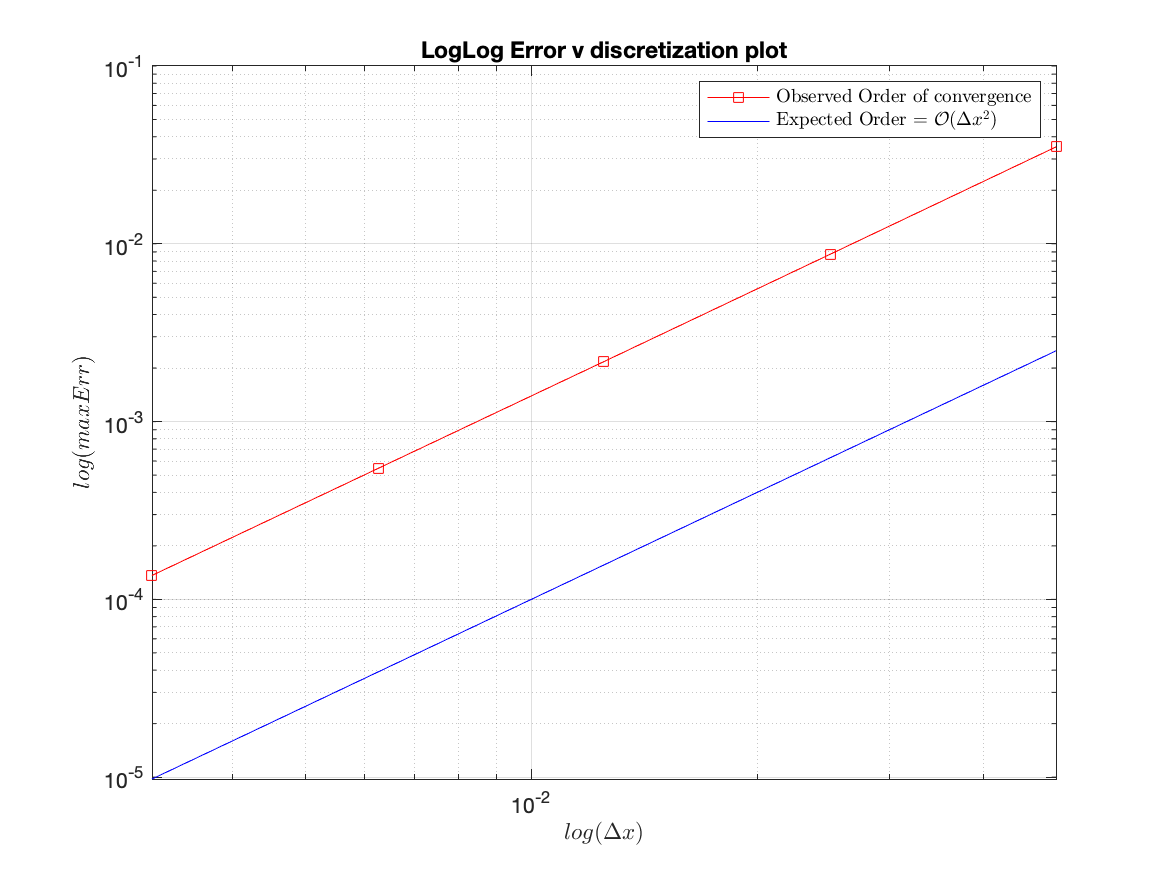
\includegraphics[width=4in]{Q1_ErrPlot_RK4.png}
        \caption{2nd order convergence for center difference scheme with RK4 time integration}
        \label{fig:Q1_ErrPlot2}
    \end{figure}    
    \end{enumerate}

  %%%%%
  %%%%%
  %%%%%
  \item {\color{red}(10 pts.) Consider the scalar conservation equation}
    \[
      u_t+[f(u)]_x=0,
    \]
    {\color{red}for $|x|<\infty$, $t>0$, and $u(x,0) = u_0(x)$. For each of the following flux functions $f(u)$}
    \[
      f(u) = 2u^4, \qquad \qquad f(u) = e^{2u}
    \]
    \begin{enumerate}
      %%%
      %%%
      %%%
      \item {\color{blue}Determine a formula for the propagation speed $S$ of a discontinuity between two states $u_L$ and $u_R$ (L and R for left and right respectively).}\\
      Using chain rule, the PDE can be written as,
      \begin{align*}
          u_t + \frac{df}{du}u_x =& \ 0 \\
      \end{align*}
      Now, the characteristics are given by $\frac{dx}{dt} = \frac{df}{du}$.
      In case of discontinuities, if the PDE is integrated over an interval $[a,b]$ containing the discontinuity, then
      \begin{align*}
          \frac{d}{dt}\int_a^b u\ dx =& \ \frac{d}{dt}\int_a^{s(t)} u\ dx + \frac{d}{dt}\int_{s(t)}^b u\ dx  \\
          =& \ \int_a^{s(t)}u_t\ dx + \frac{ds}{dt}u(s^{-},t) + \int_{s(t)}^b u_t\ dx - \frac{ds}{dt}u(s^{+},t) \\
          =& \ \int_a^{s(t)}-\bra{f(u)}_x\ dx + \frac{ds}{dt}u(s^{-},t) + \int_{s(t)}^b -\bra{f(u)}_x\ dx - \frac{ds}{dt}u(s^{+},t) \\
          =& \ -\bra{f(u)}|_a^b + \left[f(u)\right] - \left[u\right]\frac{ds}{dt} \\
          \cancel{\frac{d}{dt}\int_a^b u\ dx} =& \ \cancel{-\bra{f(u)}|_a^b} + \left[f(u)\right] - \left[u\right]\frac{ds}{dt}
      \end{align*}
      Therefore, speed of discontinuity is given by $\frac{ds}{dt}=\frac{[f]}{[u]} $ across discontinuity.
      %%%
      %%%
      %%%
      \item {\color{blue}Determine the speed $S$ when $u_L = 2$, and $u_R=1$.}\\
      Case 1: $f(u) = 2u^4$
      \begin{align*}
          \frac{ds}{dt} =& \frac{f(u_R)-f(u_L)}{u_R-u_L} \\
          =& \ \frac{2u_R^4 - 2u_L^4}{u_R - u_L} = \frac{2-2^5}{-1} = 30
      \end{align*}
      Case 2: $f(u)=e^{2u}$
      \begin{align*}
          \frac{ds}{dt} =& \frac{f(u_R)-f(u_L)}{u_R-u_L} \\
          =& \ \frac{e^{2u_R}-e^{2u_L}}{u_R-u_L} = \frac{e^2-e^4}{-1} = e^4 - e^2
      \end{align*}
    \end{enumerate}

  %%%%%
  %%%%%
  %%%%%
  \item {\color{red}(20 pts.) Consider the conservation equation from \#2 above with $f(u) = e^{2u}$.}
    \begin{enumerate}
      %%%
      %%%
      %%%
      \item {\color{blue}Find the characteristic form of the equation. What is the characteristic speed?} \\
      Characteristic form of the equation is, 
      \begin{align*}
          \frac{dx}{dt} =& \ \frac{df}{du} \\
          x(t) =& \ \frac{df}{du}t + x_0 \\
          x_j(t) =& \ 2e^{2u_j}t + x_j
      \end{align*}
      where, the characteristic speed is $\frac{df}{du} = 2e^{2u}$.
      %%%
      %%%
      %%%
      \item {\color{blue}Assuming $u_0(x)=\frac{1}{2}(u_L+u_R)+\frac{1}{2}(u_R-u_L)\tanh(10x)$, use the characteristics, and the fact that $u$ is constant along characteristics, to sketch qualitative solutions at various times for the following 2 cases;} \\
      The characteristic solutions at several final times are plotted in Fig~\ref{fig:csolution}. The initial conditions ($u_L $ and $u_R$) are mentioned in the figure's title.

      \begin{enumerate}
        \item $u_L=-1$, $u_R=1$.
        \item $u_L=1$, $u_R=-1$.
      \end{enumerate}
      \begin{figure}[htp]
      	\centering
	\begin{tabular}{cc}
	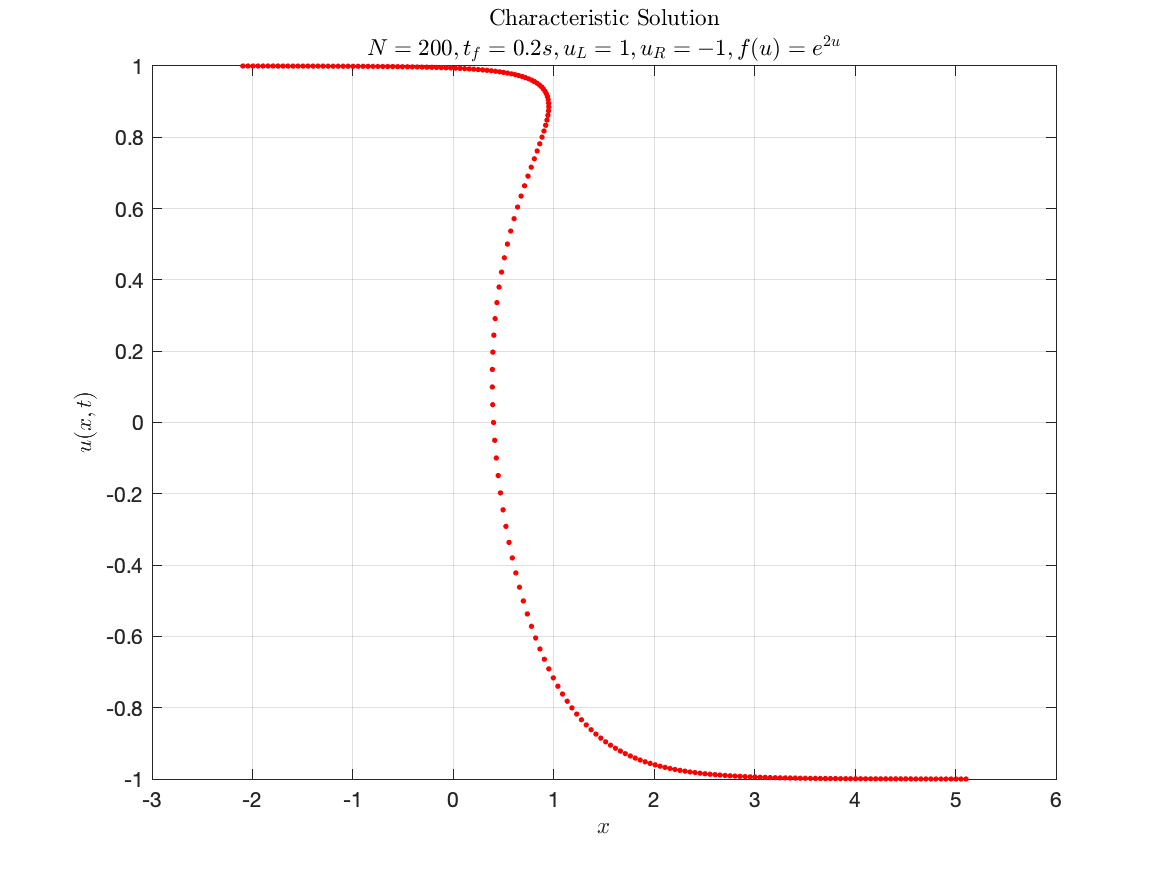
\includegraphics[width=3.4in]{Q2charac_1.png} & 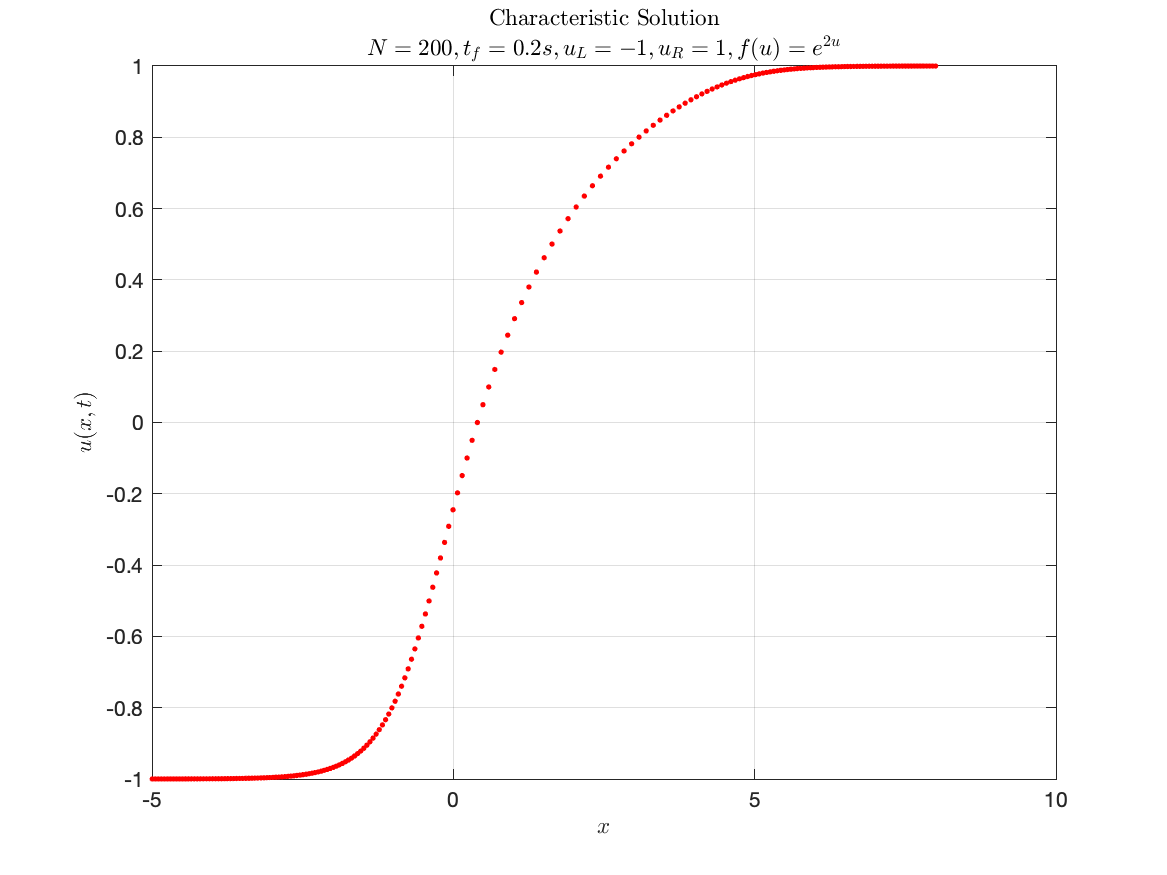
\includegraphics[width=3.4in]{Q2charac_2.png}\\
	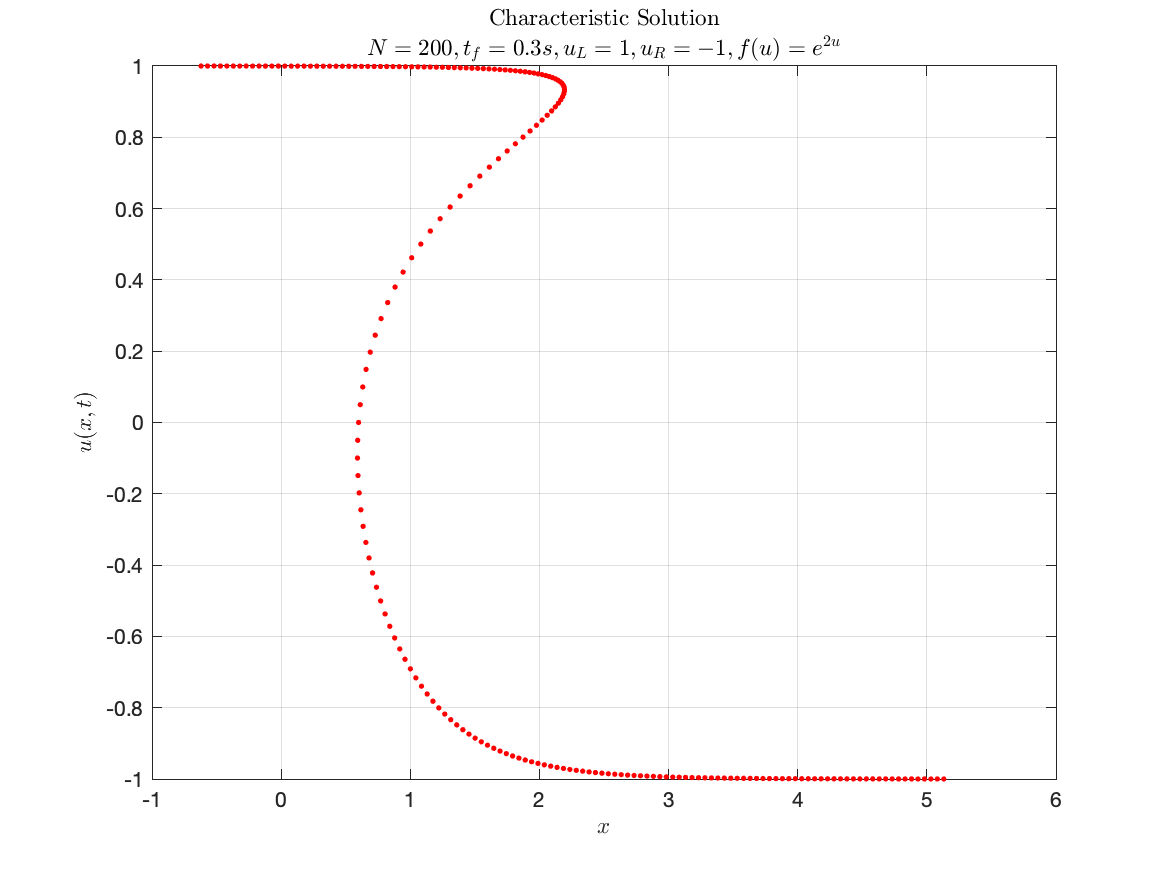
\includegraphics[width=3.4in]{Q2charac_3.png} & 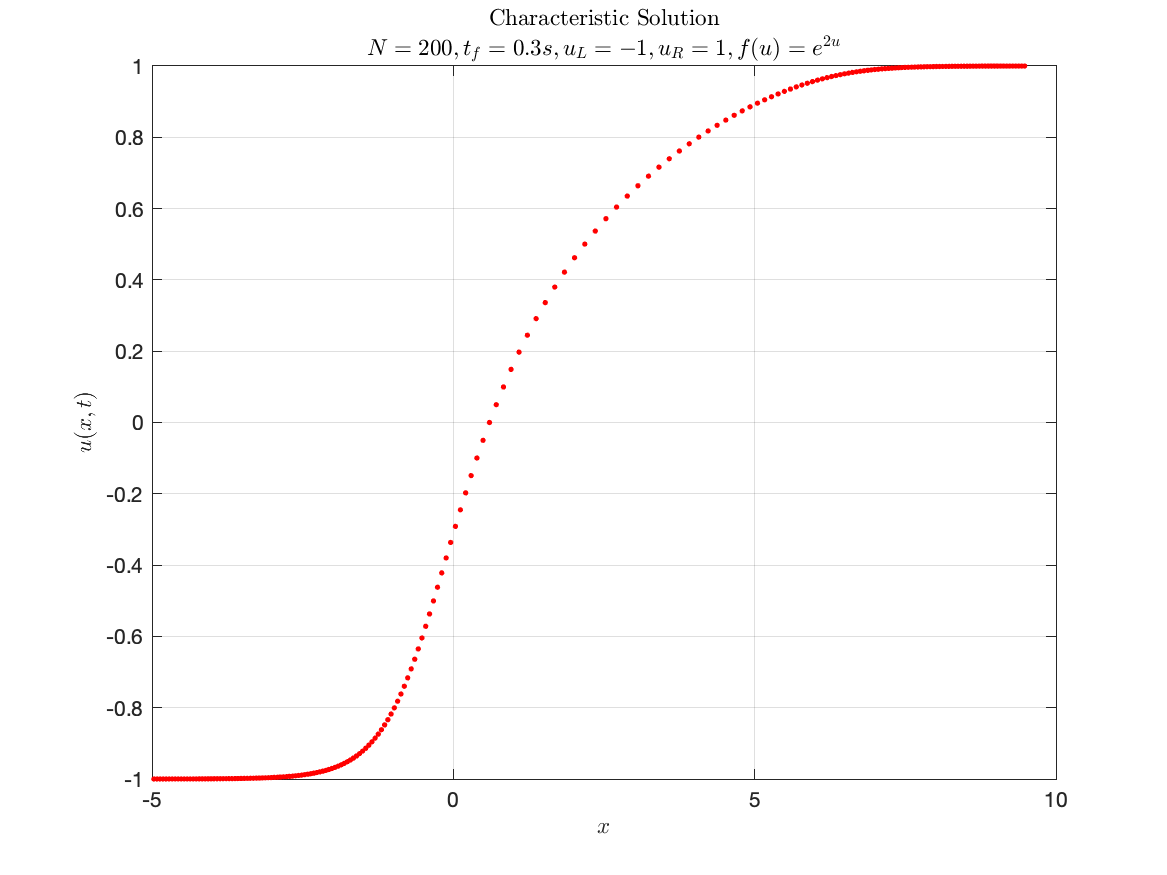
\includegraphics[width=3.4in]{Q2charac_4.png}\\
	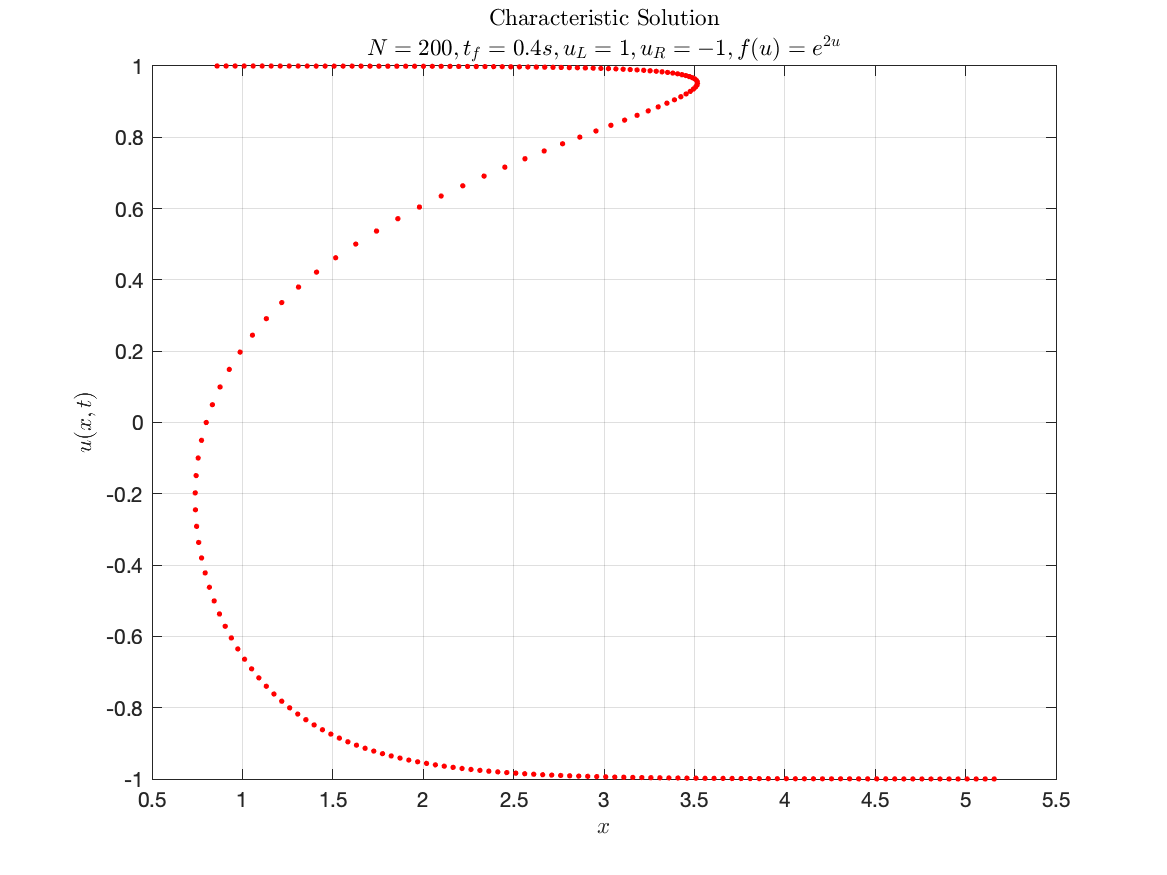
\includegraphics[width=3.4in]{Q2charac_5.png} & 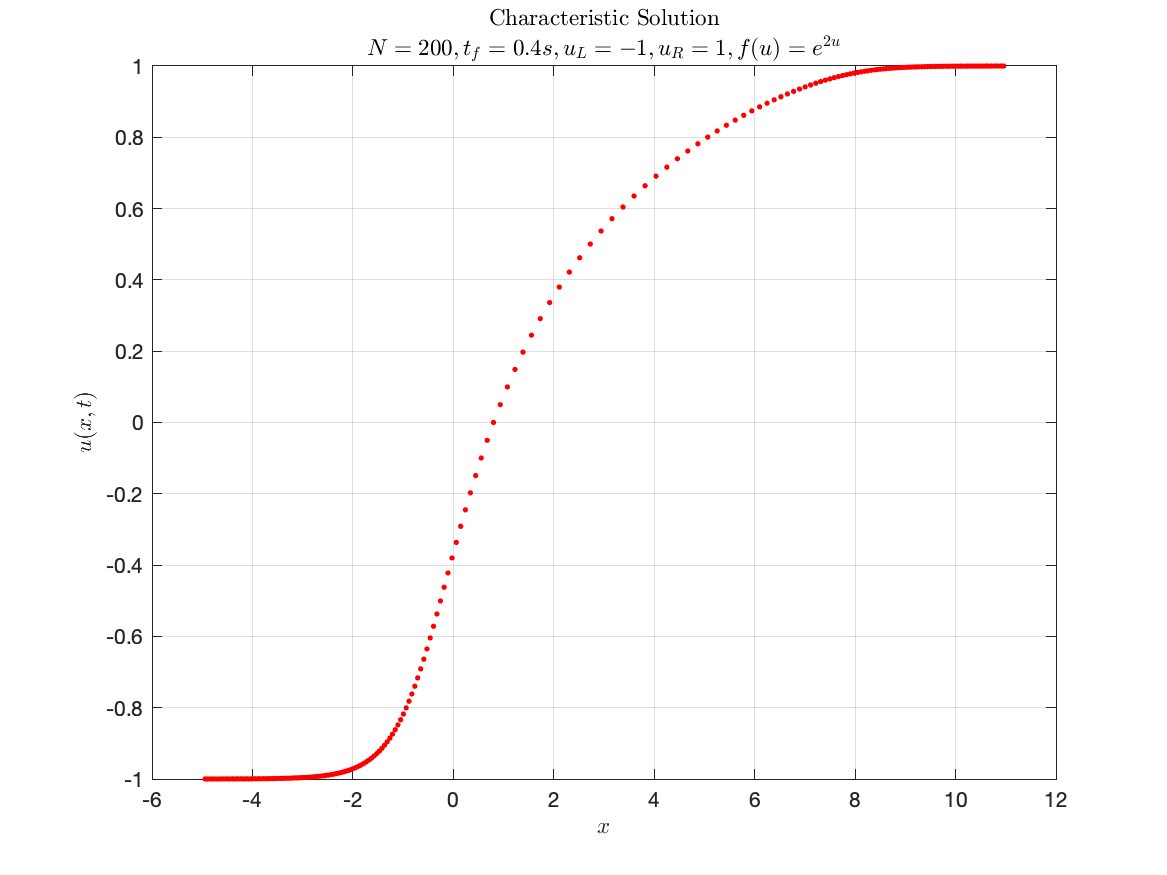
\includegraphics[width=3.4in]{Q2charac_6.png}
	\end{tabular}
	\caption{Characteristic Solutions at different final times}
	\label{fig:csolution}
      \end{figure}
      %%%
      %%%
      %%%
      \item {\color{blue}Write a conservative upwind code and verify your predictions from (b) above.}\\
      The code for a conservative upwind scheme is attached below in Listing~\ref{lst:NL_Cons}. The solutions are plotted in Fig~\ref{fig:nsolution}. 
      \begin{figure}[htp]
      	\centering
	\begin{tabular}{cc}
	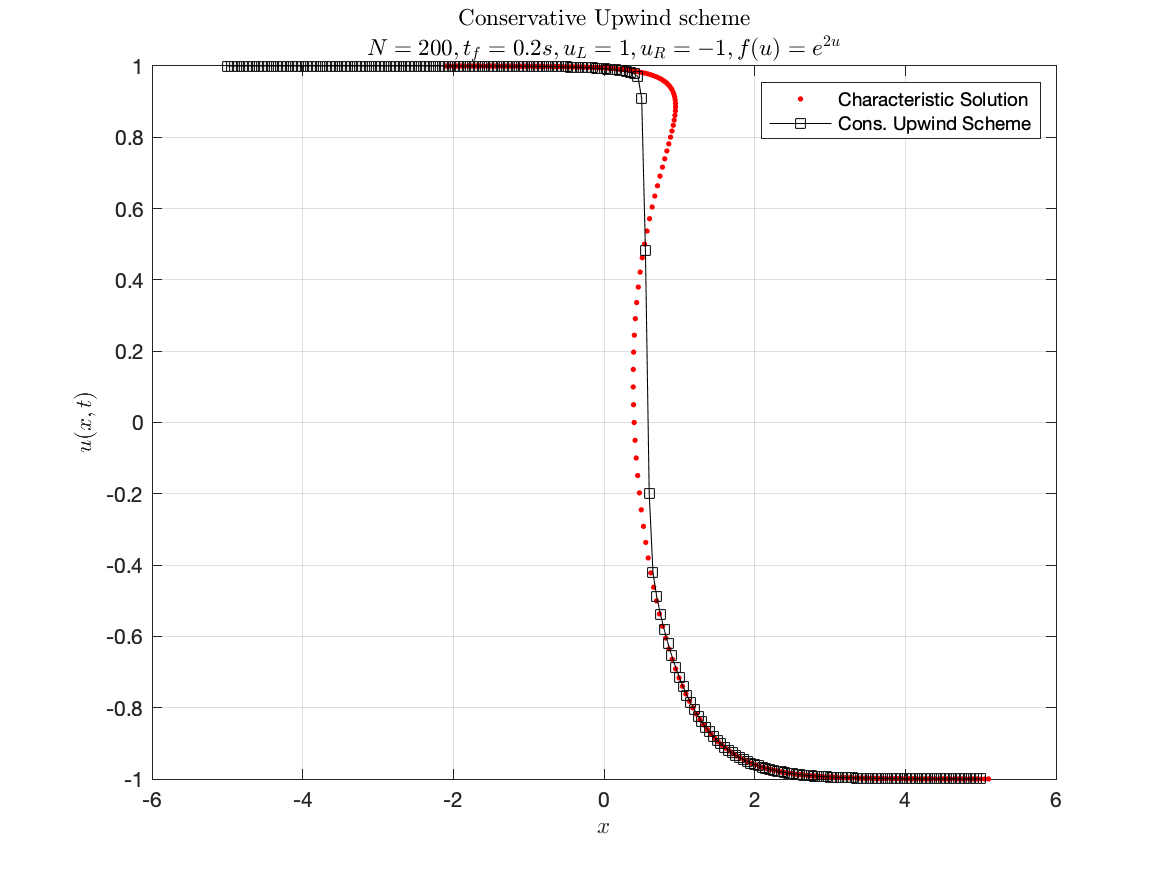
\includegraphics[width=3.4in]{Q2_1.png} & 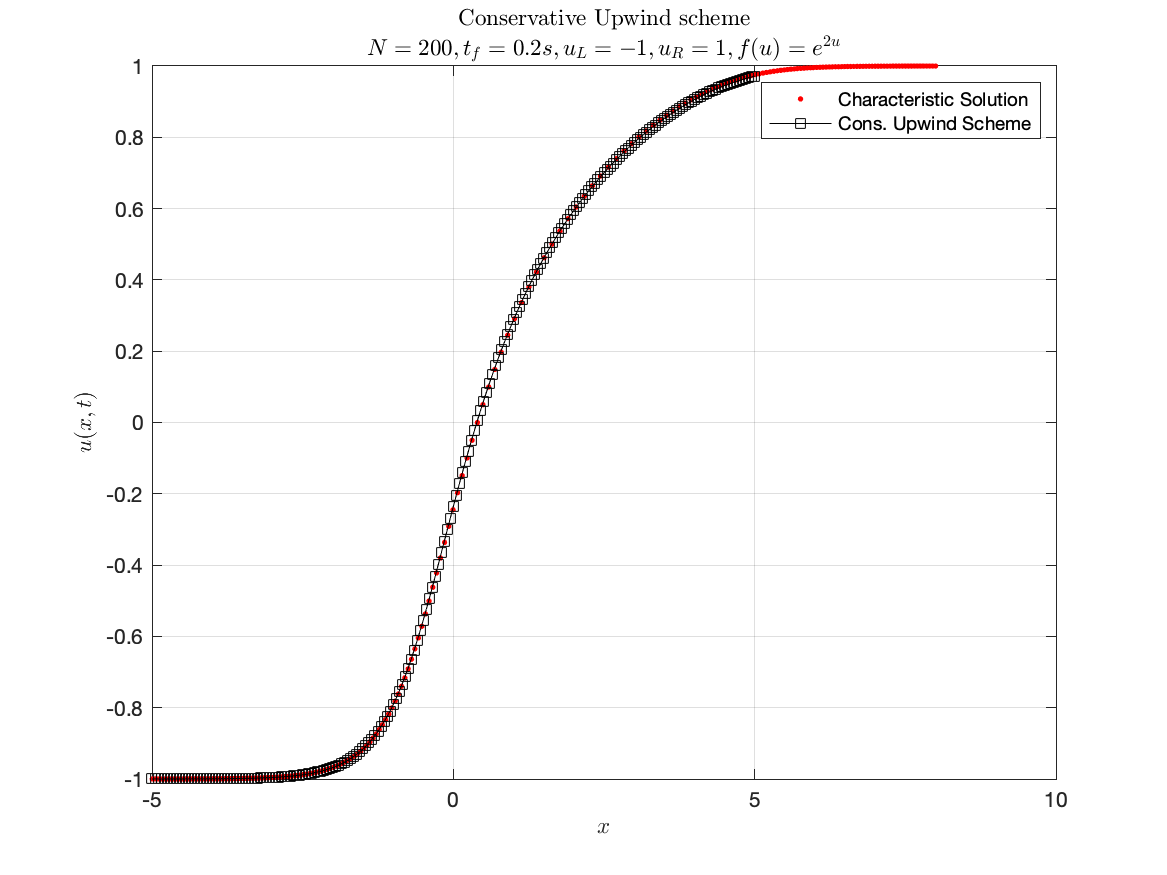
\includegraphics[width=3.4in]{Q2_2.png}\\
	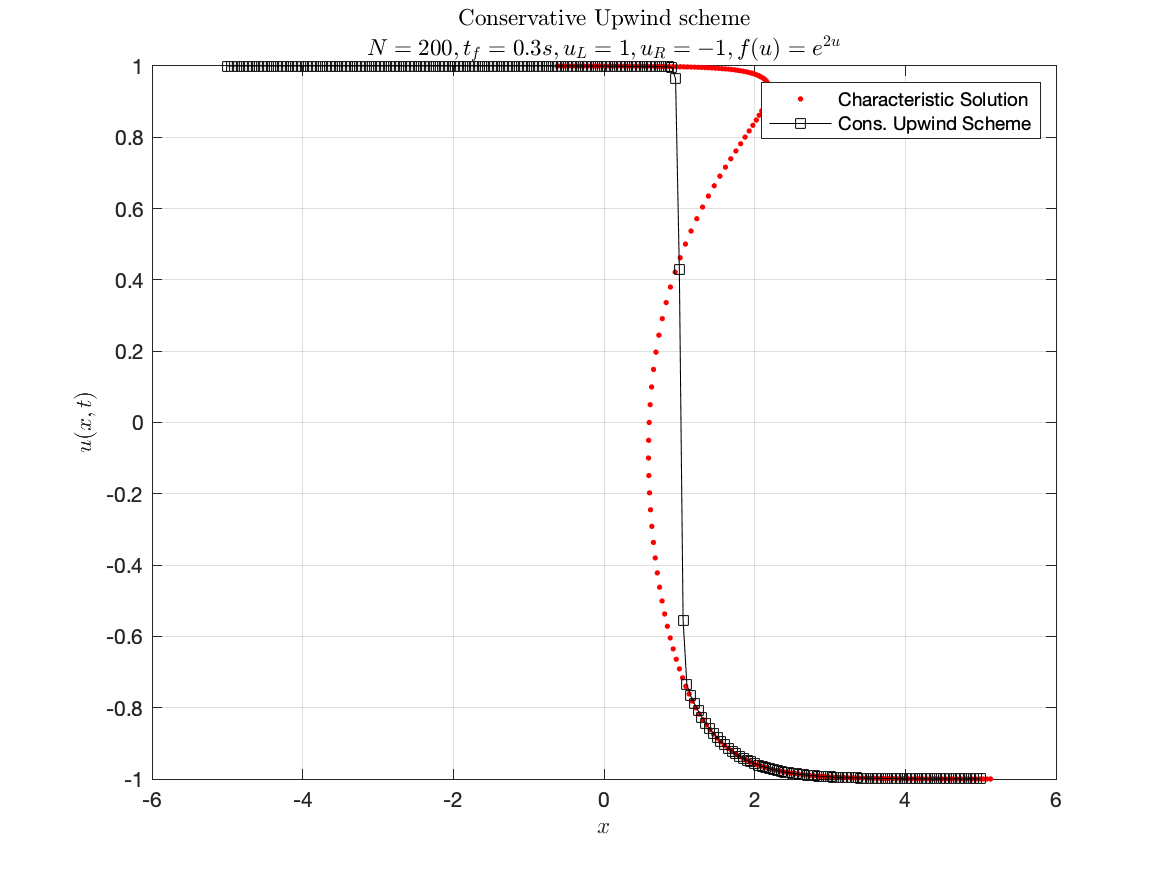
\includegraphics[width=3.4in]{Q2_3.png} & 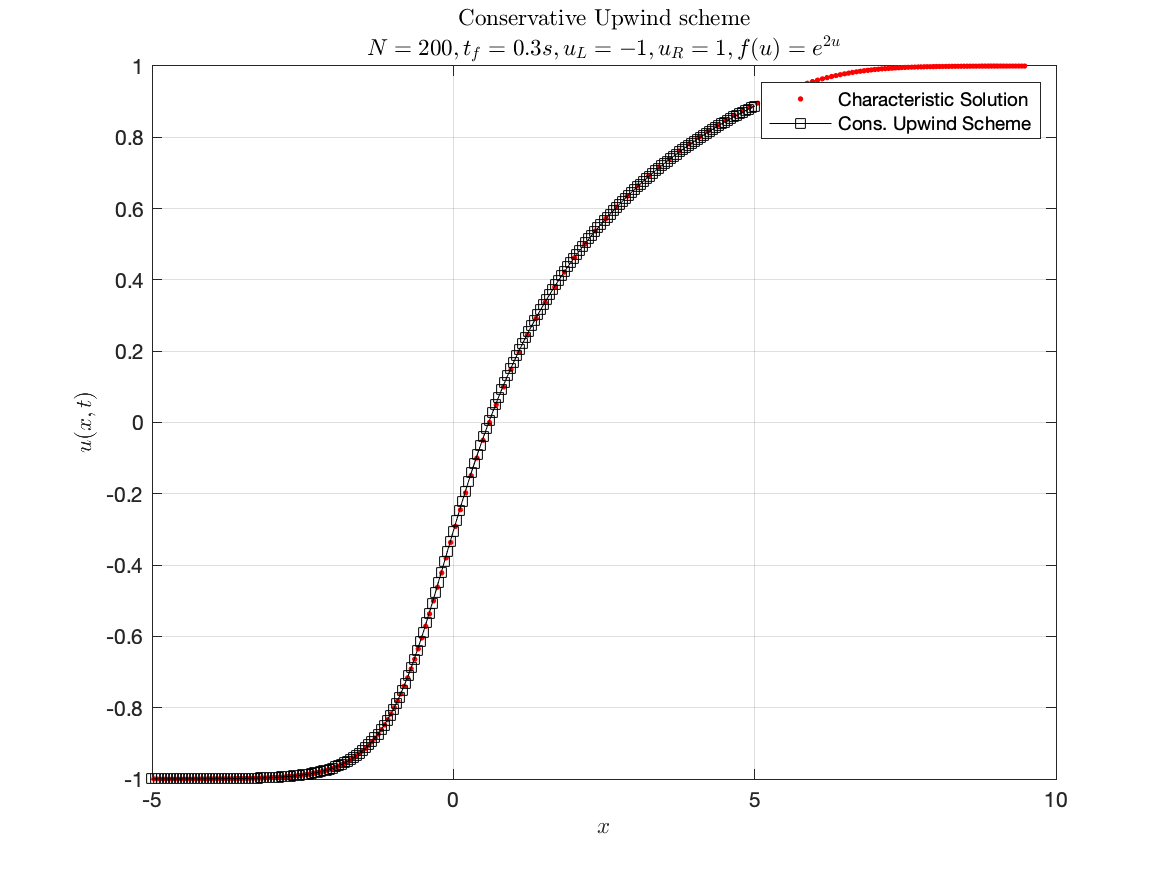
\includegraphics[width=3.4in]{Q2_4.png}\\
	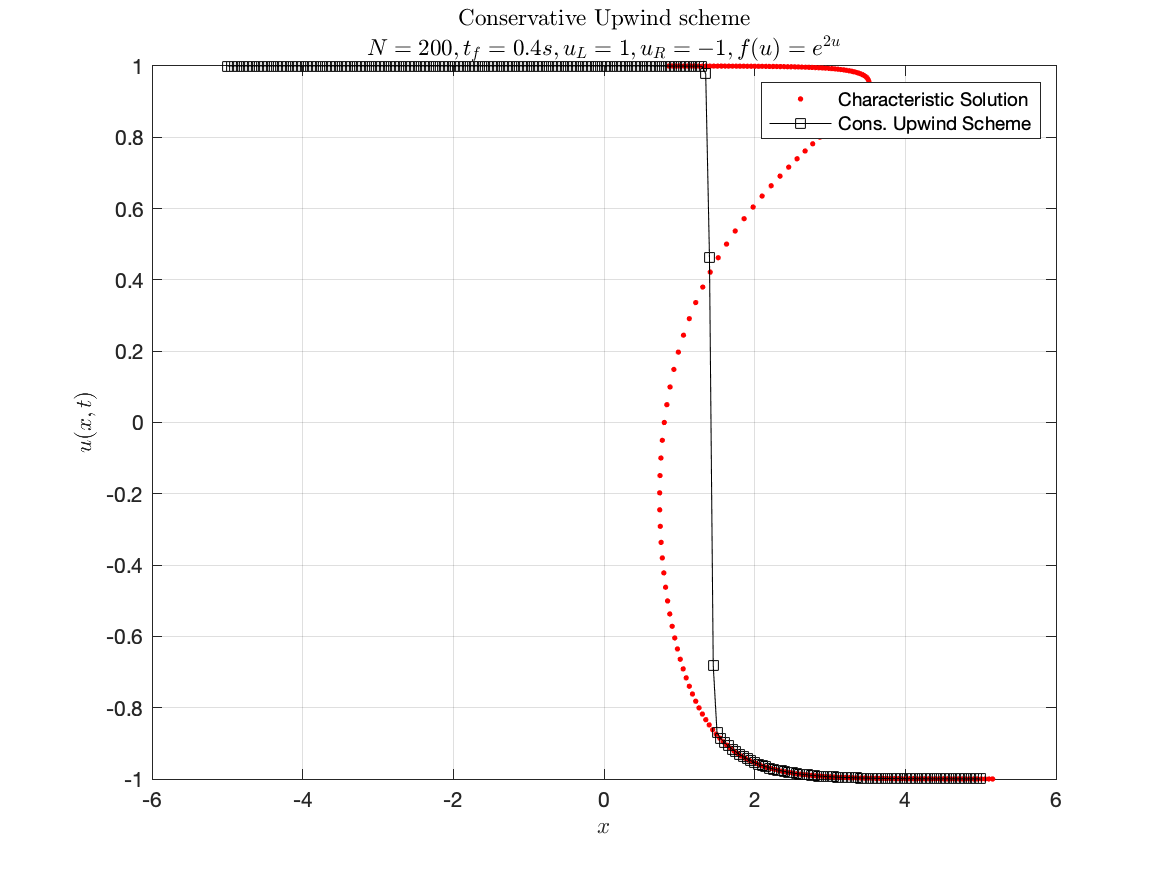
\includegraphics[width=3.4in]{Q2_5.png} & 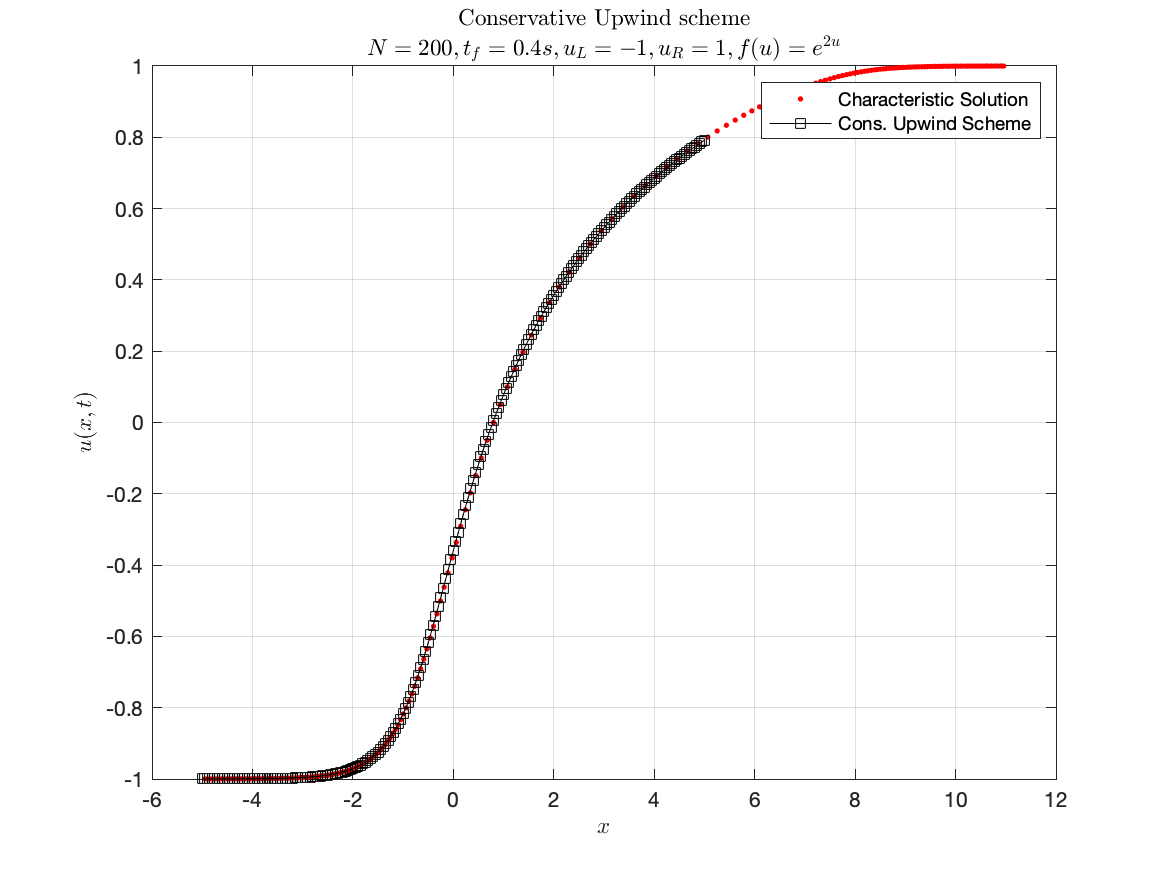
\includegraphics[width=3.4in]{Q2_6.png}
	\end{tabular}
	\caption{Upwind Scheme Solutions at different final times}
	\label{fig:nsolution}
      \end{figure}
      \lstinputlisting[caption={Conservative Upwind scheme for Nonlinear PDE}, label={lst:NL_Cons}, language=Matlab]{NonlinearConservation.m}
      %%%
      %%%
      %%%
    \end{enumerate}

\end{enumerate}

The script used to generate the plots is attached in Listing~\ref{lst:pscript}.
\lstinputlisting[caption={Script to generate plots},label={lst:pscript}, language=Matlab]{script2.m}

\end{document}
